\documentclass{beamer}
\usepackage{../common_slides}
\usepackage{tikz-qtree}
\usepackage{pdfpages}
% \usepackage{enumitem}

\title{A Tour of Natural Language Applications}
\date{}
\author{CS 287 }
\begin{document}

\begin{frame}
  \titlepage
\end{frame}

\begin{frame}{AlphaGo}
  \begin{center}
    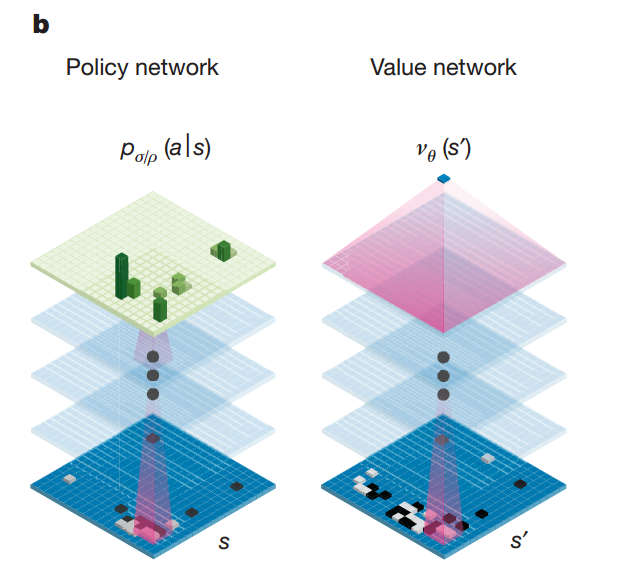
\includegraphics[height=0.7\textheight]{alphago}
  \end{center}
\end{frame}

\begin{frame}{Review: LSTM (Hochreiter and Schmidhuber, 1997)}
  \begin{center}
    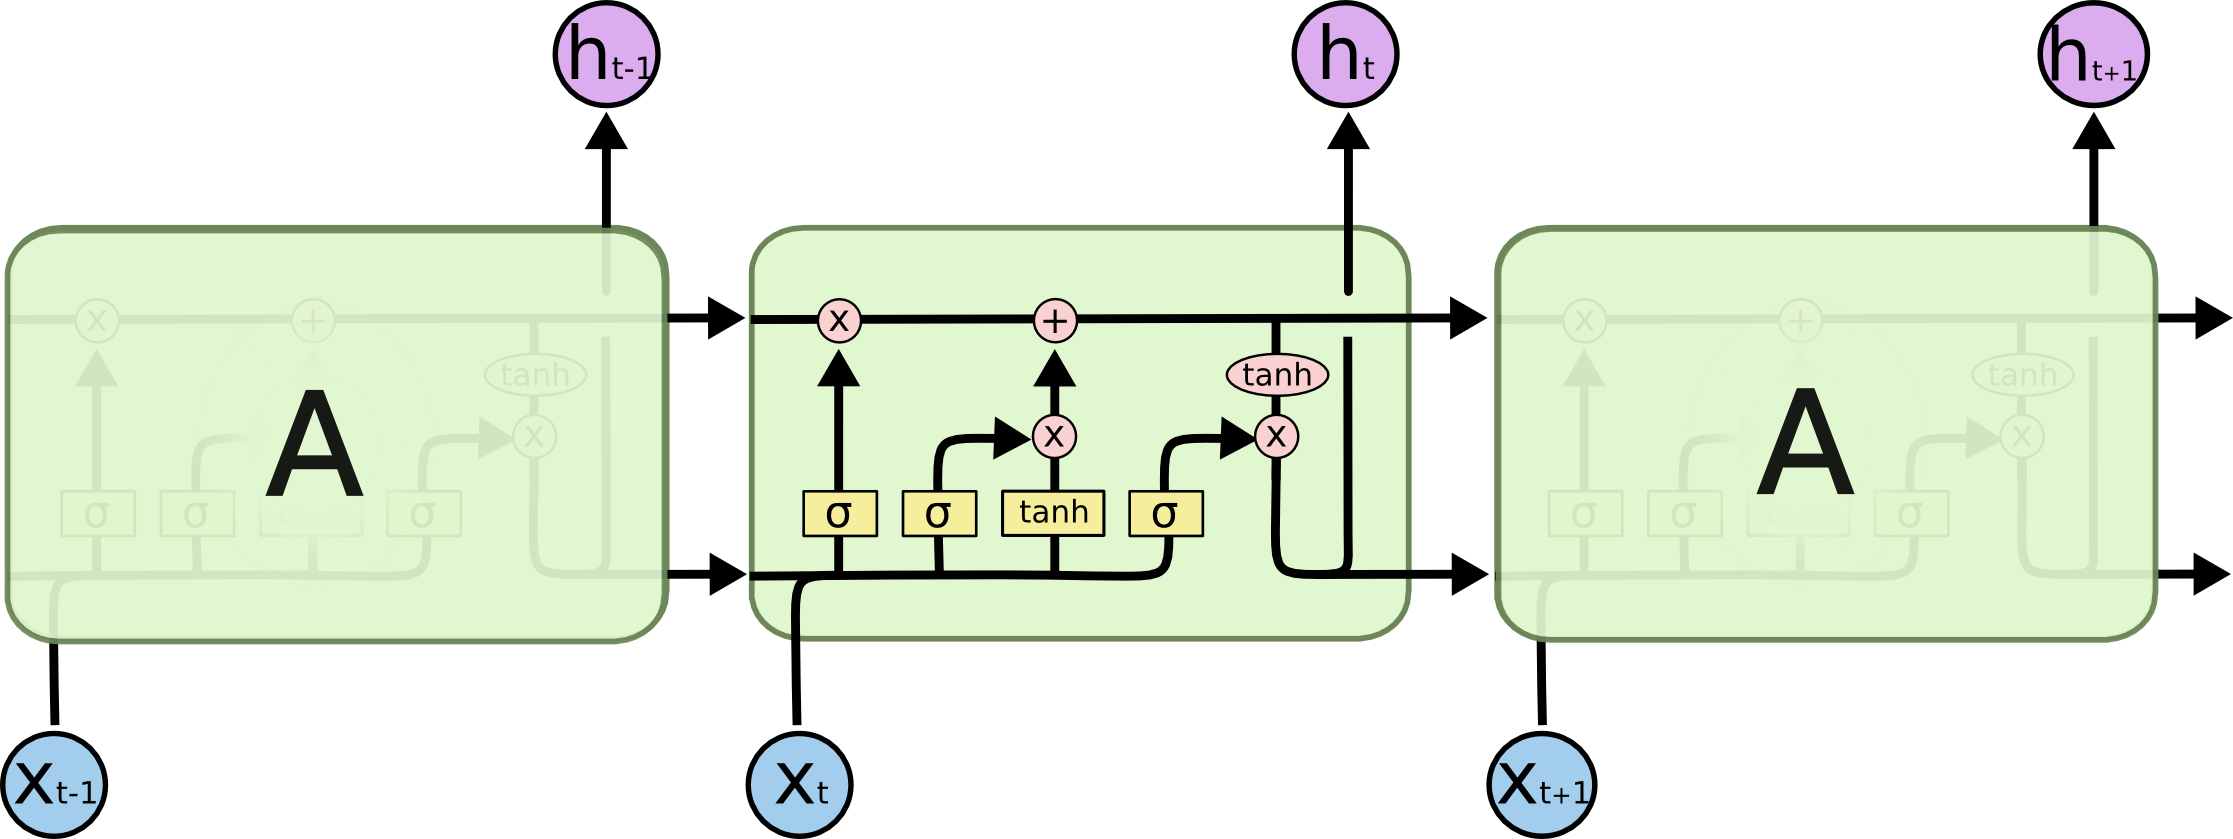
\includegraphics[width=\textwidth]{LSTM3-chain}
  \end{center}
\end{frame}

\begin{frame}{Review: Highway Network (Srivastava et al., 2015)}
  \begin{itemize}
  \item Now add a combination at each dimension.
  \item $\odot$ is point-wise multiplication. 
  \end{itemize}
  \begin{eqnarray*}
    NN_{highway}(\boldx) &=& (1-\boldt) \odot \tilde{\boldh} + \boldt \odot \boldx \\
    \tilde{\boldh} &=& \relu(\boldx \boldW^1 + \boldb^1) \\
    \boldt &=& \sigma(\boldx \boldW^t + \boldb^t) \\
    \boldW^t, \boldW^1 &\in& \reals^{\dhid \times \dhid} \\
    \boldb^t, \boldb^1 &\in& \reals^{1 \times \dhid} 
  \end{eqnarray*}
  \begin{itemize}
  \item $\tilde{\boldh}$; \textit{transform} (e.g. standard MLP layer)
  \item $\boldt$; \textit{carry} (dimension-specific dynamic skipping)
  \end{itemize}
\end{frame}


\begin{frame}{Review: Gated Recurrent Unit (GRU) (Cho et al 2014)}
    \begin{eqnarray*}
      R(\bolds_{i-1}, \boldx_i) &=& (1-\boldt) \odot \tilde{\boldh} + \boldt \odot \bolds_{i-1} \\
      \tilde{\boldh} &=& \tanh(\boldx \boldW^x + (\boldr \odot \bolds_{i-1})  \boldW^s + \boldb)  \\
      \boldr &=& \sigma(\boldx \boldW^{xr} + \bolds_{i-1}\boldW^{sr} + \boldb^r) \\
      \boldt &=& \sigma(\boldx \boldW^{xt} + \bolds_{i-1}\boldW^{st} + \boldb^t) \\
      \boldW^{xt}, \boldW^{xr}, \boldW^{x} &\in& \reals^{\din \times \dhid} \\
      \boldW^{st}, \boldW^{sr}, \boldW^{s} &\in& \reals^{\dhid \times \dhid} \\
      \boldb^t, \boldb &\in& \reals^{1 \times \dhid} \\
    \end{eqnarray*}

    \begin{itemize}
    \item $\boldt$; dynamic skip-connections
    \item $\boldr$; reset gating
    \item $\bolds$; hidden state
    \item $\tilde{\boldh}$; gated MLP
    \end{itemize}
\end{frame}

\begin{frame}{Review: Long Short-Term Memory}
  Finally, another output gate is applied to $\boldh$
    \begin{eqnarray*}
      R(\bold \bolds_{i-1}, \boldx_i) &=& [\boldc_i, \boldh_i]  \\
      \boldc_i &=& \boldj \odot \boldi  + \bold f \odot \bold c_{i-1}    \\
      \boldh_i &=& \tanh(\boldc_i) \alert{\odot \boldo}\\ 
      \boldi &=& \tanh(\boldx \boldW^{xi} + \boldh_{i-1}\boldW^{hi} + \boldb^i) \\
      \boldj &=& \sigma(\boldx \boldW^{xj} + \boldh_{i-1}\boldW^{hj} + \boldb^j) \\
      \boldf &=& \sigma(\boldx \boldW^{xf} + \boldh_{i-1}\boldW^{hf} + \boldb^f) \\
      \boldo &=& \sigma(\boldx \boldW^{xo} + \boldh_{i-1}\boldW^{ho} + \boldb^o) \\
    \end{eqnarray*}
\end{frame}

\begin{frame}{Review: The Promise of RNNs}
  \begin{itemize}
  \item Learn the long-range interactions of language from data.
    \air 

  \item Example: classify true and false statements:
    \pause 

  \item \textbf{Example:}
    \air 

    \structure{\texttt{Eliot house is the coolest}}
    \air 
    
    \alert{\texttt{Mather does not look like a prison.}}
    \air 
    
  \item Works well if you control for \textit{exploding} or \textit{vanishing} gradients.
  \end{itemize}
\end{frame}


\begin{frame}{Quiz}
  Last class we discussed the issue of 
  the exploding gradient in RNNs. 
  
  There are two practical heuristics  
  for this problem:
  \begin{itemize}
  \item gradient clipping, i.e. bounding any gradient
    by a maximum value 
  \item gradient normalization, i.e. renormalizing the 
    the RNN gradients if they are above a fixed norm 
    value.
  \end{itemize}

  \air 

  Describe the positive and negatives of these approaches.
  How would you implement these in a system like Torch?  
\end{frame}

\begin{frame}{Today's Lecture}
  \begin{itemize}
  \item High-level picture of select natural language challenges.
    \air

  \item Caveat: Not a representative sample of NLP.
    
    \air

  \item Meant as a final project shopping list.
  \end{itemize}
\end{frame}

\begin{frame}{Recommendations}
  \begin{itemize}
  \item Sometimes datasets are private, speak to us about getting them. 
    \air

  \item The state-of-the-art on these problems is changing quite quickly.
    \air 
    
  \item Getting Started: 
    \air 
    \begin{itemize}
    \item Make sure you understand the problem and the metric.
      \air
    \item Read papers on the topic.
      \air
    \item Experiment first with count-based or linear models
      \air
    \item Reimplement other systems
    \end{itemize}
  \end{itemize}
\end{frame}

\begin{frame}{Topics}
  High-level areas:
  \begin{itemize}
  \item Information Extraction
    \begin{itemize}
    \item Named-Entity Recognition
    \item Semantic-Role Labeling
    \item Entity Linking
    \end{itemize}
    \air 
  \item Question Answering
    \begin{itemize}
    \item Knowledge Graph (factoid)
    \item Knowledge Processing (non-factoid)
    \item Comprehension (non-factoid)
    \end{itemize}
  \item Document Understanding
    \begin{itemize}
    \item Discourse
    \item Summarization
    \item Coreference
    \end{itemize}
  \end{itemize}

\end{frame}

\begin{frame}{Other NLP Areas}
  There are many other areas of NLP:
  \begin{itemize}
  \item Speech
  \item Syntax
  \item Machine Translation
  \end{itemize}
  \air
  Require more details [future lectures]

  \air 
  Other possible topics (bring-your-own domain knowledge)
  \begin{itemize}
  \item Music Processing
  \item Vision
  \item Game Playing
  \end{itemize}
\end{frame}

\section{Information Extraction}

\begin{frame}
  \begin{center}
    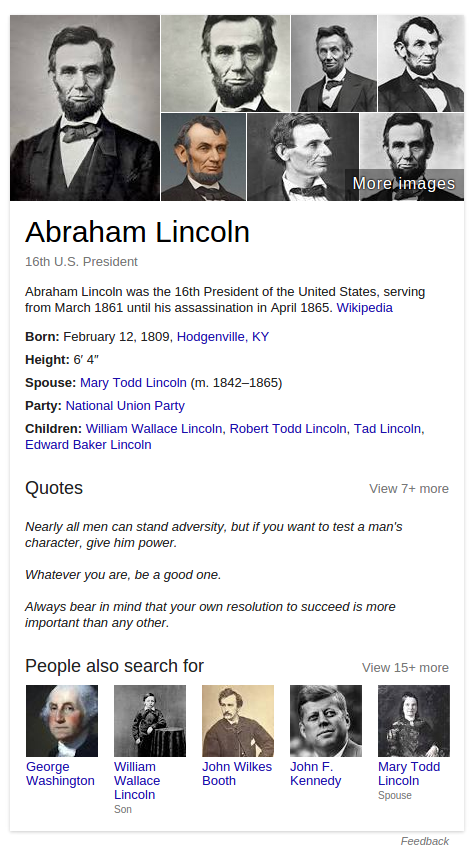
\includegraphics[height=\textheight]{abelincoln}
  \end{center}
\end{frame}

\begin{frame}{Information Extraction}
  \textbf{Goal:} Map text to structured information.
  \air 

  \textbf{Applications:} 
  \begin{itemize}
  \item Knowledge-base construction
    \air 
  \item Quantitative research from freetext
    \air 
  \item Identifying relationships 
  \end{itemize}
\end{frame}


\begin{frame}{Terminology (ACE 2008 task)}
  \begin{description} \itemsep 20pt
    
  \item[Entity] the underlying semantic actor.
    \begin{itemize}
    \item e.g. persons, countries, organizations, teams
    \end{itemize}
   
  \item[Relation] semantic relations between entities
    \begin{itemize}
    \item e.g. part of, located in, member of, works for
    \end{itemize}

  \item[Event] a semantic occurrence involving entities
    \begin{itemize}
    \item e.g. marriage, attack, takeover, visit
    \end{itemize}

  \item[Mention] a reference to an entity, relation, or event in text
    \begin{itemize}
    \item e.g. China, the country, it, the People's Republic of China
    \end{itemize}
  \end{description}
\end{frame}

\begin{frame}{Problem 1: Named-Entity Recognition}
  \begin{description} \itemsep 20pt
  \item[Goal] Identify explicitly named entities in text.
  \item[Input] Sentence to be tagged. 
  \item[Output] Mentions of identified entities and their type. 
  \end{description}  

\end{frame}

\begin{frame}{Named-Entity Recognition}
  \textbf{Input:} \texttt{U.N. official Ekeus heads for Baghdad. }
  \air
  
  \textbf{Gold:} \texttt{ [ORG \alert{U.N.} ] official [PER \structure{Ekeus} ] heads for [LOC \alert{Baghdad} ] .  } 
\end{frame}

\begin{frame}[fragile]{Standard Dataformat (CoNLL 2003)}
  \begin{center}
    

\begin{verbatim}
   U.N.         NNP  I-NP  I-ORG 
   official     NN   I-NP  O 
   Ekeus        NNP  I-NP  I-PER 
   heads        VBZ  I-VP  O 
   for          IN   I-PP  O 
   Baghdad      NNP  I-NP  I-LOC 
   .            .    O     O 
\end{verbatim}
  \end{center}
\end{frame}

\begin{frame}{BIO Tagging}
  \begin{description} \itemsep 20pt
  \item[B-TYPE] Stop current mention and begin new mention
    \air 
  \item[I-TYPE] Continue adding to current mention
  \item[O ] Not part of a mention.
  \end{description}
  \pause
  
  \textbf{Example:} 

  \texttt{ [PER \alert{George Bush} ]  [LOC \structure{U.S.} ] president is traveling to [LOC \alert{Baghdad} ] .  } 
\end{frame}

\begin{frame}{Example Tag Set}
  \begin{itemize}
  \item Loc
  \item Org
  \item Person
  \item Misc 
  \end{itemize}
  \air 
  
  \begin{itemize}
  \item How big is $\mcC$ for this problem?
  \end{itemize}
\end{frame}

\begin{frame}{Problem 2: Entity Linking}
  \begin{description} \itemsep 20pt
  \item[Goal] Identify explicit entities and link to a standard
  central database.
  \item[Input] Sentence or Document
  \item[Output] Mentions and pointer to a central source.
  \end{description}  

\end{frame}


\begin{frame}{Entity Linking: Wikification (TAC 2014)}
  \begin{itemize}
  \item Uses Wikipedia as canonical source.

    \air
  \item Goal is to link mentions to the correct wikipedia page. 

    \air
  \item Classification is over a much larger space. 
  \end{itemize}
\end{frame}


\begin{frame}{Wikification (Roth et al, 2014)}
  \begin{center}
    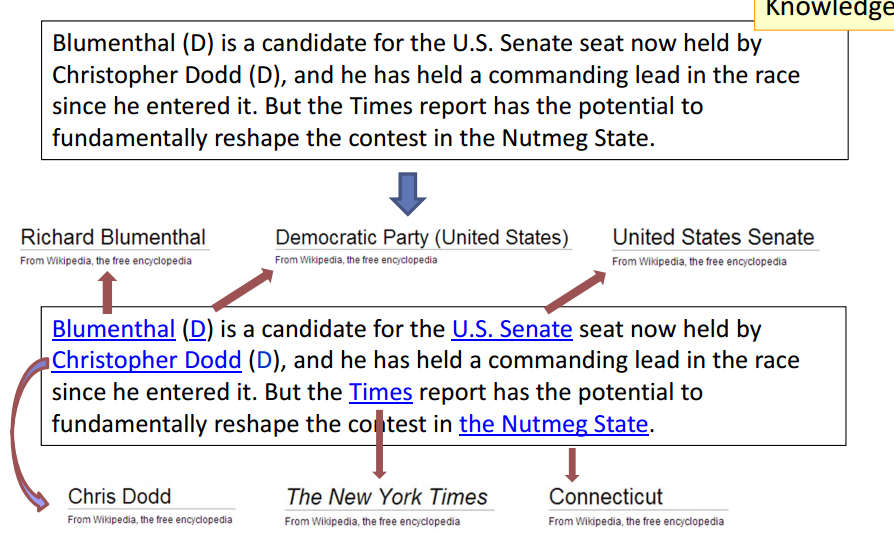
\includegraphics[width=\textwidth]{wikification}
  \end{center}
\end{frame}

\begin{frame}{Medical Term Linkage (Semeval, 2015) }
  \begin{itemize}
  \item Uses canonical medical thesaurus (SNOMED/UMLS)
    \air 
  \item Goal is to link medical notes to thesaurus
    \air 

  \item Subset of UMLS has order of 100,000 terms.
  \end{itemize}
\end{frame}

\begin{frame}{Medical Term Extraction}

  \begin{enumerate}
  \item The rhythm appears to be [ \alert{atrial fibrillation} ].  
  \item The [ \alert{left atrium} ] is moderately [ \alert{dilated} ] .  
  \item 53 year old man s/p [ \alert{fall from ladder} ].
  \end{enumerate}

  Linked terms:
  \begin{itemize}
  \item atrial fibrillation - C0004238; UMLS preferred term ``atrial fibrillation''
  \item left atrium...dilated - C0344720; UMLS preferred term ``left atrial dilatation''
  \item fall from ladder - C0337212; UMLS preferred term is ``accidental fall from ladder''  
  \end{itemize}
\end{frame}

% \begin{frame}{SemEval 14}
%   \url{http://alt.qcri.org/semeval2015/task14/index.php?id=task-description}
% \end{frame}

\begin{frame}{Problem 3: Semantic Role Labeling}
  \begin{description} \itemsep 20pt
  \item[Goal] Mark the semantic roles of sentence elements
  \item[Input] Sentence
  \item[Output] Identify verb, its type, its arguments, and their types
  \end{description}  
\end{frame}

\begin{frame}{Language Applications: Semantic Role Labeling }
 He  would  n't accept anything of value from those he was writing about  

 \air 

 [A0 He ] [AM-MOD would ] [AM-NEG n't ] [V accept ] [A1 anything of value ] from [A2 those he was writing about ] 

 \begin{itemize}
 \item V: verb (accept)
 \item A0: acceptor 
 \item A1: thing accepted 
 \item A2: accepted-from 
 \item A3:attribute 
 \item AM-MOD: modal 
 \item  AM-NEG: negation
 \end{itemize}
\end{frame}

\begin{frame}{SRL Requires Long-Range Interactions}
  Collobert approach:
  \begin{itemize}
  \item   First given a verb $w_i$ e.g. \texttt{accept}.
    \air 
  \item  Then consider a word $w_j$ e.g. \texttt{n't}
    \air
  \item  For a word $w_k$ features are 
    \[v(w_k), v_2(cap(w_k)), v_3(i-k), v_4(j-k)\]

    \air
  \item Convolution over sentence is used to predict role.
    \air 
  \item $O(n \times |verbs|)$ convolutions per sentence
  \end{itemize}
\end{frame}

\section{Question Answering}

\begin{frame}{Question Answering}
  \begin{itemize}
  \item Big area, lots of different problems.
    \air 
  \item Generally specific to the type of question and style of input. 
    \air 

    \texttt{what high school did president bill clinton attend?}
    
    versus 
    
    \texttt{how many rivers in texas are longer than the red?}
    \air 

  \item Various methods for solving:
    \begin{itemize}
    \item Learn to map text to explicit logical query
    \item Treat logical query as latent term 
    \item Attempt to directly map to answer  
    \end{itemize}
  \end{itemize}
\end{frame}

\begin{frame}{Factoid Question Answering}
  \begin{description} \itemsep 20pt
  \item[Goal]Map question to an answer from a  knowledge base 
  \item[Input] Question and knowledge-base source
  \item[Output] Answer
  \end{description}  
\end{frame}

\begin{frame}[fragile]{WebQuestions (Berant )} 
\textbf{Questions:}
\begin{itemize}
\item what high school did president bill clinton attend?
\item what form of government does russia have today?
\item what movies does taylor lautner play in?
\end{itemize}

\textbf{Answers:}
\begin{itemize}
\item Hot Springs High School \url{http://www.freebase.com/view/en/bill_clinton}
\item Constitutional republic \url{http://www.freebase.com/view/en/russia}
\item  Eclipse, Valentine's Day, The Twilight Saga: Breaking Dawn -   Part 1, New Moon \url{http://www.freebase.com/view/en/taylor_lautner}
\end{itemize}
\end{frame}

\begin{frame}{Freetext Knowledge Sources}

  \begin{description} \itemsep 20pt
  \item[Goal]Map question to an answer described in text.
  \item[Input] Question and Text Source (textbooks)
  \item[Output] Answer
  \end{description}
\end{frame}


\begin{frame}{Biological Processes (Berant et al, 2013)}
  \begin{center}
    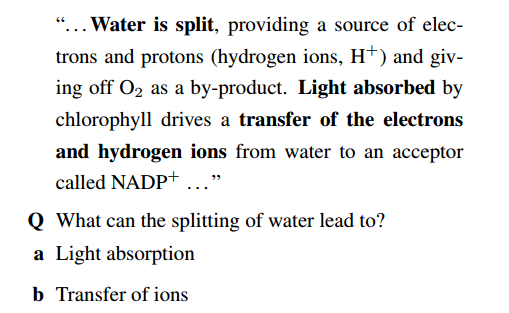
\includegraphics[width=10cm]{water}
  \end{center}
\end{frame}

% \begin{frame}{WikiQA}
  
% \end{frame}

\begin{frame}{Non-Factoid}
  \begin{description} \itemsep 20pt
  \item[Goal]Map question to an answer described in casual text.
  \item[Input] Question, multiple choices, and text source (narratives)
  \item[Output] Answer
  \end{description}  
\end{frame}

\begin{frame}{MCTest (Richardson et al, 2013)}
  James the Turtle was always getting in trouble. Sometimes he'd reach into the freezer and empty out all the food. Other times he'd sled on the deck and get a splinter. His aunt Jane tried as hard as she could to keep him out of trouble, but he was sneaky and got into lots of trouble behind her back.

  One day, James thought he would go into town and see what kind of trouble he could get into. He went to the grocery store and pulled all the pudding off the shelves and ate two jars. Then he walked to the fast food restaurant and ordered 15 bags of fries. He didn't pay, and instead headed home.

  His aunt was waiting for him in his room. She told James that she loved him, but he would have to start acting like a well-behaved turtle.After about a month, and after getting into lots of trouble, James finally made up his mind to be a better turtle.

\end{frame}

\begin{frame}{MCTest: Questions}
  \begin{itemize}
   

  \item What is the name of the trouble making turtle?
    \begin{enumerate}
    \item Fries  \item Pudding \item James \item Jane
    \end{enumerate}
    \item What did James pull off of the shelves in the grocery store?
      \begin{enumerate}
      \item  pudding \item fries \item food \item splinters
      \end{enumerate}
    \item Where did James go after he went to the grocery store?
      \begin{enumerate}
      \item  his deck \item his freezer \item a fast food restaurant \item
        his room
      \end{enumerate}
  \end{itemize}
\end{frame}

\begin{frame}[fragile]{bAbI Tasks (Weston et al, preprint) }
\begin{verbatim}
  1 Mary moved to the bathroom.
  2 John went to the hallway.
  3 Where is Mary?        bathroom        1
  4 Daniel went back to the hallway.
  5 Sandra moved to the garden.
  6 Where is Daniel?      hallway 4
  7 John moved to the office.
  8 Sandra journeyed to the bathroom.
  9 Where is Daniel?      hallway 4
  10 Mary moved to the hallway.
  11 Daniel travelled to the office.
  12 Where is Daniel?     office  11
\end{verbatim}
\end{frame}

\section{Document Understanding}

\begin{frame}{Discourse Parsing}
  \begin{description} \itemsep 20pt
  \item[Goal] Determine the discourse relation between adjacent sentences
  \item[Input] Two sentences 
  \item[Output] One of a predefined set of relationship, e.g. compare, contrast expand.
  \end{description}  

\end{frame}

\begin{frame}{Implicit Discourse Connectives (PDTB)}
  \texbf{Questions:}
  \begin{itemize}
  \item \alert{Financial planners often urge investors to diversify and to
    hold a smattering of international securities.} \structure{And many emerging
    markets have outpaced more mature markets, such as the U.S. and
    Japan.}
  \item \alert{Country funds offer an easy
    way to get a taste of foreign stocks without the hard research of
    seeking out individual companies.} \structure{ But it doesn’t take much to get
    burned.  }
  \item \alert{But it doesn’t take
    much to get burned.} \structure{FOR EXAMPLE Political and currency
    gyrations can whipsaw the funds.}
  \end{itemize}

  \texbf{Answers:}
  \begin{itemize}
  \item Expansion.Conjunction 
  \item Comparison.Contrast 
  \item Expansion.Restatement.Specification
  \end{itemize}
\end{frame}

\begin{frame}{Summarization}
  \begin{description} \itemsep 20pt
  \item[Goal] Produce a shorter version of the input.
  \item[Input] Document
  \item[Output] Extracted sentences representing the document.
  \end{description}  

\end{frame}

\begin{frame}[fragile]{Document Summarization (DUC 2003)}
   Tension between Turkey and Syria has risen to
the point where the top Turkish military commander says the two
hostile neighbors have reached ``a state of undeclared war.''

   ``We are trying to be patient,'' said the commander, Gen.
Huseyin Kivrikoglu, ``but that has a limit.''

   Syria has reacted angrily to Turkey's blossoming friendship with
Israel. It also makes territorial claims against Turkey and accuses
Turkey of unfairly diverting water from rivers that flow through
both countries.

   For its part, Turkey is complaining ever more loudly about
Syria's support for Kurdish insurgents in Turkey. The insurgents
are said to have bases in Syria, and their leader reportedly lives
in Damascus.

   Turkey and Syria are moving troops and equipment to border
positions, according to news reports, but no outbreak of fighting
is considered imminent.

\end{frame}

% \begin{frame}{Summarization Result}

%   \begin{itemize}
%   \item 

%   Tensions between Turkey and Syria have reached a point causing the top Turkish military commander to say 
% they have reached "a state of undeclared war".                                                          

%   \item Turkey accuses Syria of supporting Kurdish rebels in Turkey, a charge denied by Syria.

%   \item Syria is angry over Turkey's closer ties to Israel and alleges that Turkey, by building dams on the Euphr
% ates River, threatens its water supply.
                                                                 
%   \item Egypt's President Mubarak has visited Saudi Arabia and Damascus and plans to continue to Ankara hoping to
%  defuse the crisis. 
                                                                                     
%   \item Israel claims "no part" in the tension. 

%   \item  Turkey has attacked Kurdish bases in Iraq and threatens those in Syria.
%   \end{itemize}
% \end{frame}


\begin{frame}{Sentence Summarization}
  \begin{description} \itemsep 20pt
  \item[Goal] Shorter version of the original sentence.
  \item[Input] Sentence
  \item[Output] Shortened sentence (possibly with different words).
  \end{description}  
\end{frame}




\begin{frame}{Sentence Summarization and Compression}
  \begin{center}
    \textbf{Source}
  \end{center}
    
  \begin{figure}
    \textit{\structure<2>{Russian Defense Minister Ivanov}
      called \structure<3>{Sunday} for the creation of
      a joint front \structure<4>{for combating} global terrorism. }
  \end{figure}

  \begin{center}
    \textbf{Target}
  \end{center}

  \begin{figure}
    \centering
    \textit{\structure<2>{Russia} calls for joint
      front \structure<4>{against} terrorism.}
  \end{figure}

\air
\air

\textbf{Summarization Phenomena:} 

\begin{itemize}
\item<2-> \alert<2>{Generalization}
\item<3-> \alert<3>{Deletion}
\item<4-> \alert<4>{Paraphrase}
% \item<5-> \alert<5>{Tense}
\end{itemize}
\end{frame}
\begin{frame}
  
\includegraphics[width=\linewidth]{ap}
\end{frame}


\begin{frame}{Coreference}
  \begin{description} \itemsep 20pt
  \item[Goal] Cluster mentions based on their underlying entity.
  \item[Input] Document
  \item[Output] Clusters of coreferent mentions.
  \end{description}  
\end{frame}




{
\setbeamercolor{background canvas}{bg=}
\includepdf[pages=2-4]{swacl15}
}

\end{document}
